%%%%%%%%%%%%%%%%%%%%%%%%%%%%%%%%%%%%%%%%%%%%%%%%%%%%%%%%%%%%%%%%%
%%%%%%%%%%%%%%%%%%%%%%%%%%%%%%%%%%%%%%%%%%%%%%%%%%%%%%%%%%%%%%%%%
\section{Introduction}
%%%%%%%%%%%%%%%%%%%%%%%%%%%%%%%%%%%%%%%%%%%%%%%%%%%%%%%%%%%%%%%%%
%%%%%%%%%%%%%%%%%%%%%%%%%%%%%%%%%%%%%%%%%%%%%%%%%%%%%%%%%%%%%%%%%

{\tt B2.5} was originally a structured code with a rectangular topology and has been developed as such for
more than 30 years. Eventually, it was decided to move to an unstructured finite volume solver. The main reason
is that it was impossible to model up to the real vessel walls with a rectangular grid topology, while maintaining acceptable grid quality.
Extending the {\tt B2.5} mesh up to the real vessel walls has many advantages:

\begin{itemize}
\item First wall fluxes can be computed.
\item The distribution of recycling sources along the walls is much more realistic.
\item {\it Ad hoc} radial plasma boundary conditions (leakage / decay lengths) are no longer needed.
\item Fluid neutrals can be modelled further down in the divertor, closer to where the pumps are typically located
(or at least to where the pumps are located in \SOLPSITER simulations).
\end{itemize}

The move to the unstructured finite volume solver and extended grids is described in full in the 2021 NME paper of W. Dekeyser {\it et al.} \cite{DEKEYSER2021}.

%%%%%%%%%%%%%%%%%%%%%%%%%%%%%%%%%%%%%%%%%%%%%%%%%%%%%%%%%%%%%%%%%
%%%%%%%%%%%%%%%%%%%%%%%%%%%%%%%%%%%%%%%%%%%%%%%%%%%%%%%%%%%%%%%%%
\section{Discretization}
%%%%%%%%%%%%%%%%%%%%%%%%%%%%%%%%%%%%%%%%%%%%%%%%%%%%%%%%%%%%%%%%%
%%%%%%%%%%%%%%%%%%%%%%%%%%%%%%%%%%%%%%%%%%%%%%%%%%%%%%%%%%%%%%%%%

This section explains the discretization on the unstructured finite volume grid. The content of this section is copied from Ref. \cite{DEKEYSER2021}.

Figure \ref{fig:mesh_angles} describes a cell face separating two control volumes:
\begin{figure}[hbtp]
\ifpdf
    \centerline{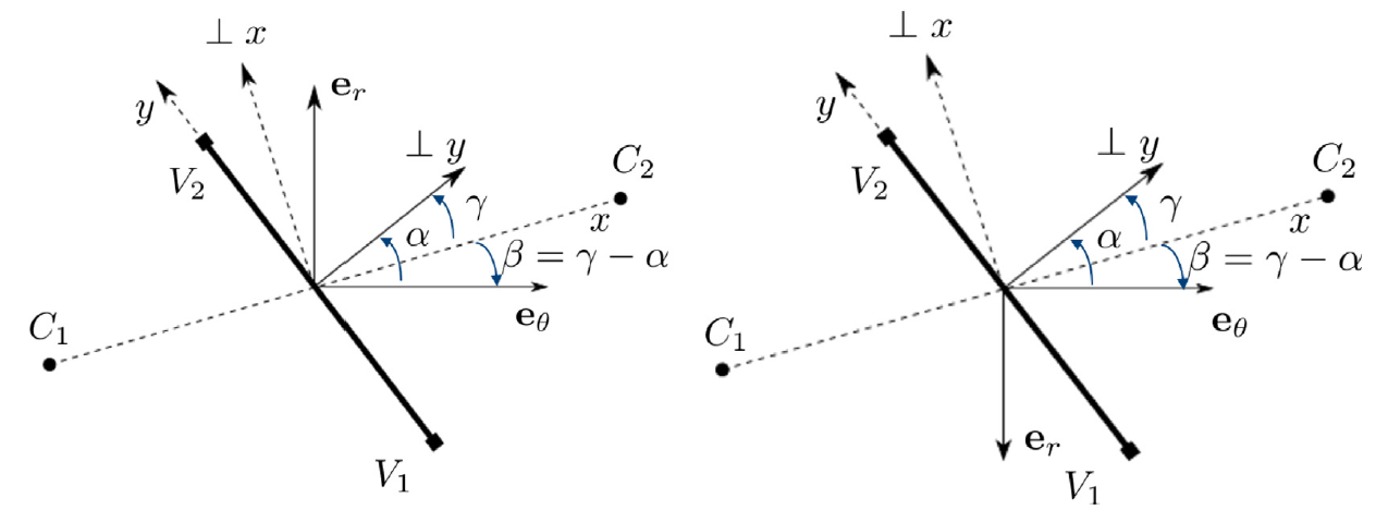
\includegraphics[width=14cm]{FiguresWG/mesh_angles.png}}
\else
    \centerline{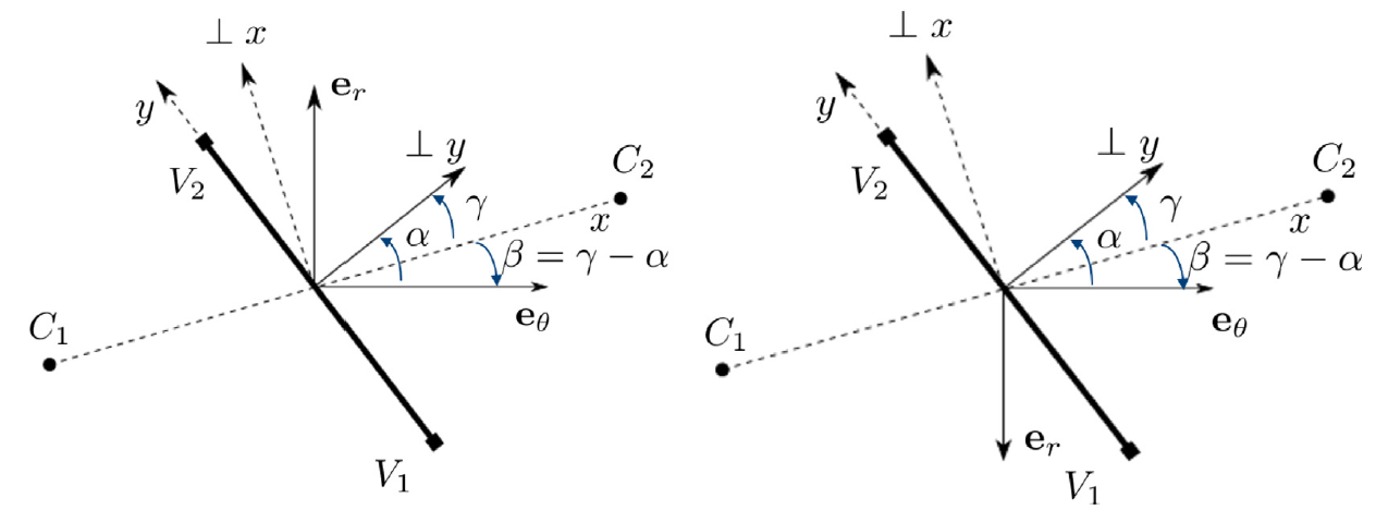
\includegraphics[width=14cm]{FiguresWG/mesh_angles.eps}}
\fi
    \caption{Local coordinate systems defining cell face orientation w.r.t. magnetic field, cell centers, and vertices. Left: toroidal field out of page. Right: toroidal field into the page.
    Figure reproduced from \cite{DEKEYSER2021}.}
    \label{fig:mesh_angles}
\end{figure}

The definitions of the variables in Figure \ref{fig:mesh_angles} are as follows:

\begin{itemize}
\item {\tt $C_1$} is the center of control volume 1. The index for that control volume is given by {\tt fcCv(iFc,1)}.
\item {\tt $C_2$} is the center of control volume 2. The index for that control volume is given by {\tt fcCv(iFc,2)}.
\item {\tt $V_1$} is the first vertex of the face. Its index is given by {\tt fcVx(iFc,1)}.
\item {\tt $V_2$} is the second vertex of the face. Its index is given by {\tt fcVx(iFc,2)}. The convention is that, when we look from {\tt $V_1$} to {\tt $V_2$}, {\tt $C_1$} is on the left and {\tt $C_2$} is on the right.
\item {\tt x} The $x$-direction is defined through the (not necessarily straight)
coordinate line connecting {\tt $C_1$} and {\tt $C_2$}, going through the center of the
cell face, and positive from {\tt $C_1$} to {\tt $C_2$}.
\item {\tt y} The $y$-direction is tangent to the face, positive from {\tt $V_1$} to {\tt $V_2$}.
\item {\tt $\alpha$} is the included angle between the magnetic field vector and the face normal.
{\tt fcQalf(iFc,0)} is the cosine of {\tt $\alpha$} and {\tt fcQalf(iFc,1)} is the sine of {\tt $\alpha$}.
\item {\tt $\gamma$} is the included angle between the cell-connector vector and the normal vector
of face {\tt iFc}. {\tt fcQgam(iFc,0)} is the cosine of {\tt $\gamma$} and {\tt fcQgam(iFc,1)} is the sine of {\tt $\gamma$}. It will hold that {\tt 0.lt.fcQgam(,).le.1}.
\item {\tt $\beta$} is the included angle between the cell-connector and the magnetic field vector.
{\tt fcQbet(iFc,0)} is the cosine of {\tt $\beta$} and {\tt fcQbet(iFc,1)} is the sine of {\tt $\beta$}.
\item {\tt fcHc(iFc,1)} is the distance between {\tt $C_1$} and the cell face center. {\tt fcHc(iFc,2)} is the distance between {\tt $C_2$} and the cell face center.
\item {\tt fcHt(iFc)} is the distance between {\tt $V_1$} and {\tt $V_2$}.
\end{itemize}

The flux of a particular quantity $u$ follows a convection-diffusion prescription:

\begin{equation*}
\mathbf{\Gamma} = \mathbf{C} u - \mathcal{D} \nabla u
\end{equation*}

The anisotropy in the equations is most naturally expressed w.r.t.
the poloidal ($\theta$) and radial ($r$) directions, which, by definition, are locally
orthogonal to each other. In our notation, the poloidal direction
points along the poloidal projection of the magnetic field, and the
radial direction is orthogonal to it in the poloidal plane, forming a
right-handed system with the third unit vector along the toroidal
projection of the field. These unit vectors therefore may flip orientation
with poloidal/toroidal field reversal. The coefficient
$\mathbf{C} = C_\theta \mathbf{e}_\theta + C_r \mathbf{e}_r$ is a vector describing the convective
flux of $u$, with components
defined in the poloidal and radial directions, and $\mathcal{D} = [D_{\theta \theta} D_{\theta r}, D_{r \theta} D_{r r}]$
is a diffusive tensor. The cross-diffusivities are included
because they are representative of the treatment of drift flows.
The {\tt B2.5} finite volume technique requires the evaluation of the fluxes across
cell faces:

\begin{align*}
 \mathbf{\Gamma} \cdot \mathbf{S} & = \Gamma_\theta S_\theta + \Gamma_r S_r \\
 & = \left( C_\theta u - D_{\theta \theta} \nabla_\theta u - D_{\theta r} \nabla_r u \right) S_\theta +
 \left( C_r u - D_{r \theta} \nabla_\theta u - D_{r r} \nabla_r u \right) S_r,
 \end{align*}

where $\mathbf{S} = S_\theta \mathbf{e}_\theta +  S_r \mathbf{e}_r $
is the surface vector of a face, expanded in its
poloidal and radial components.

To compute the poloidal and radial components of the gradient,
we relate them to the gradients in the $x$ and $y$
directions, which in turn can be computed directly from differences
between cell center (for $\nabla_\theta$) and vertex (for $\nabla_r$) values of $u$. The
desired expression for the components of the gradient can be obtained
by expanding the gradient in the orthogonal poloidal-radial system,
$\nabla u = \nabla_\theta u \cdot \mathbf{e}_\theta + \nabla_r u \cdot \mathbf{e}_r$,
and applying the definition of the gradient, $\nabla_d u = \nabla u \cdot \mathbf{d}$
for an arbitrary direction $\mathbf{d}$, to the unit vectors $\mathbf{e}_\theta$ and
$\mathbf{e}_r$:

\begin{align*}
\nabla_x u & = \nabla u \cdot \mathbf{e}_x = \nabla_\theta u \mathbf{e}_\theta \cdot \mathbf{e}_x + \nabla_r u \mathbf{e}_r \cdot \mathbf{e}_x, \\
\nabla_y u & = \nabla u \cdot \mathbf{e}_y = \nabla_\theta u \mathbf{e}_\theta \cdot \mathbf{e}_y + \nabla_r u \mathbf{e}_r \cdot \mathbf{e}_y.
\end{align*}

From Figure \ref{fig:mesh_angles} we see that $\mathbf{e}_\theta \cdot \mathbf{e}_x = \cos \beta$,
 $\mathbf{e}_r \cdot \mathbf{e}_x = \mp \sin \beta$, $\mathbf{e}_\theta \cdot \mathbf{e}_y = -\sin \alpha$
and $\mathbf{e}_r \cdot \mathbf{e}_y = \pm \cos \alpha$, with the upper signs corresponding to toroidal field
out of the page, and the lower signs with toroidal field into the page.
Inverting the system, we obtain

\begin{align*}
\nabla_\theta u & = \frac{\cos \alpha}{\cos \gamma} \nabla_x u + \frac{\sin \beta}{\cos \gamma} \nabla_y u, \\
\nabla_r u & = \pm \frac{\sin \alpha}{\cos \gamma} \nabla_x u \pm \frac{\cos \beta}{\cos \gamma} \nabla_y u.
\end{align*}

For completeness we give also the component of the gradient normal
to the face, which is needed for some boundary conditions:

\begin{equation*}
\nabla_n u = \frac{1}{\cos \gamma} \nabla_x u + \frac{\sin \gamma}{\cos \gamma} \nabla_y u,
\end{equation*}

and note, trivially, that the component tangential to the face is the
component in the $y$-direction: $\nabla_t u = \nabla_y u$.
Computing the poloidal and radial components of the gradient in
general thus requires a combination of gradients in $x$ and $y$ directions.

Drift terms can also be discretized using the expressions above. Only
the component of the drift perpendicular to a face leads to transport
across a face. Recalling that drifts have the form of a cross-diffusion
term, the net drift flow $\Gamma_d$ across a face is of the form:

\begin{equation*}
\mathbf{\Gamma}_d \cdot \mathbf{S} = - D_d \left( \nabla_r u S_\theta - \nabla_\theta u S_r \right) = \mp D_d \nabla_y u S
\end{equation*}

where we use the identity $\mathbf{S} = \left( \cos \alpha \ \mathbf{e}_\theta \pm \sin \alpha \ \mathbf{e}_r \right) S$.
Thus, net drift flow
across the face depends only on gradients along the face, while the
decomposition of the drift into its poloidal and radial components (as
required for example for the collisions with neutrals) requires again the
correct computation of the radial/poloidal gradients on each (possibly
non-aligned) face.
Using the expressions for the fluxes and derivatives on faces given
above, the governing equations can be discretized. Gradients in cell
centers are obtained through interpolation of the cell face gradients.
The discretization schemes of the structured version of the code have
been generalized to arbitrary unstructured grids. Hybrid discretization
schemes are used for the convection-diffusion flows, which are second
order in space for diffusion-dominated flows, but tend to a first-order
upwind scheme in convection-dominated flows.
The discretization schemes of the unstructured solver no longer neglect effects of misalignment
w.r.t. the magnetic field, and hence the solver is more accurate than older {\tt B2.5} versions
 even for non-extended grid cases.

Dedicated routines in {\tt \$\{SOLPSTOP\}/modules/B2.5/src/utility/} now take care of recurring numerical operations:

\begin{itemize}
\item {\tt GRAD} computes gradients of a cell-centered quantity on the cell faces, in both poloidal and radial directions.
\item {\tt GRAD\_NT} computes gradients of a cell-centered quantity on the cell faces, in both tangential and normal directions.
\item {\tt GRADC} computes gradients of a cell-centered quantity at the cell center by first computing the gradients on faces, and then interpolating back to the cell center.
\item {\tt GRADC\_DIV} computes gradients of a cell-centered quantity at the cell-center by applying the divergence theorem.
\item {\tt DIV} computes the divergence of a flow field.
\item {\tt INTFACE} interpolates a cell-centered quantity to the cell faces.
\item {\tt INTCELL} interpolates a face-based quantity to the cell centers.
\item {\tt INTVERTEX} interpolates a cell-centered quantity to the vertices.
\end{itemize}

%%%%%%%%%%%%%%%%%%%%%%%%%%%%%%%%%%%%%%%%%%%%%%%%%%%%%%%%%%%%%%%%%
%%%%%%%%%%%%%%%%%%%%%%%%%%%%%%%%%%%%%%%%%%%%%%%%%%%%%%%%%%%%%%%%%
\section{Rhie-Chow correction in unstructured code}
%%%%%%%%%%%%%%%%%%%%%%%%%%%%%%%%%%%%%%%%%%%%%%%%%%%%%%%%%%%%%%%%%
%%%%%%%%%%%%%%%%%%%%%%%%%%%%%%%%%%%%%%%%%%%%%%%%%%%%%%%%%%%%%%%%%

To avoid odd-even decoupling in the parallel direction due to the
collocated velocity and density (pressure) fields, a Rhie-Chow scheme
for compressible flow as described in Ref.~\cite{MOUKALLED2016} is implemented for the
parallel direction. The scheme is also explained in Section 8.8 and 10.2 (older versions) or 9.8 and 11.2 (newer versions) of Ref.~\cite{FERZIGER2019}.
The switches {\tt b2npco\_pcm0}, {\tt b2npco\_pcm1}, {\tt b2npht\_pcm0} and {\tt b2npht\_pcm1} determine the strength of the corrections.

%%%%%%%%%%%%%%%%%%%%%%%%%%%%%%%%%%%%%%%%%%%%%%%%%%%%%%%%%%%%%%%%%
%%%%%%%%%%%%%%%%%%%%%%%%%%%%%%%%%%%%%%%%%%%%%%%%%%%%%%%%%%%%%%%%%
\section{WG-related TODOs for this manual}
%%%%%%%%%%%%%%%%%%%%%%%%%%%%%%%%%%%%%%%%%%%%%%%%%%%%%%%%%%%%%%%%%
%%%%%%%%%%%%%%%%%%%%%%%%%%%%%%%%%%%%%%%%%%%%%%%%%%%%%%%%%%%%%%%%%

Some sections of this manual still need to be rewritten to be consistent with the unstructured solver:

\begin{itemize}
\item Appendix \ref{cha:b2wdat_iout_4} for the debugging output tracing files.
\item Appendix \ref{cha:Mladen_2}: remove, update, or integrate with another part of the manual.
\item Appendix \ref{sec:typical_BCs} for the expressions of boundary conditions.
\item Add information on creation of new extended cases. For now we refer to the {\tt 20230815\_carre2\_presentation.pdf} presentation found on the \SOLPSITER SharePoint website, in the \href{https://sharepoint.iter.org/departments/POP/CM/IMAS/SOLPS-ITER/SOLPS-ITER\%20Extended\%20Grids\%20Workshops}{SOLPS-ITER Extended Grids Workshops} directory.
\end{itemize}

%%%%%%%%%%%%%%%%%%%%%%%%%%%%%%%%%%%%%%%%%%%%%%%%%%%%%%%%%%%%%%%%%
%%%%%%%%%%%%%%%%%%%%%%%%%%%%%%%%%%%%%%%%%%%%%%%%%%%%%%%%%%%%%%%%%
\section{Converting structured cases}
%%%%%%%%%%%%%%%%%%%%%%%%%%%%%%%%%%%%%%%%%%%%%%%%%%%%%%%%%%%%%%%%%
%%%%%%%%%%%%%%%%%%%%%%%%%%%%%%%%%%%%%%%%%%%%%%%%%%%%%%%%%%%%%%%%%

Users can easily convert their existing structured cases to run with the WG code version. How to do this is explained in documents on the \SOLPSITER SharePoint website, \href{https://sharepoint.iter.org/departments/POP/CM/IMAS/SOLPS-ITER/SOLPS-ITER\%20Extended\%20Grids\%20Workshops}{SOLPS-ITER Extended Grids Workshops} directory, namely {\tt Session\_case\_conversion.pdf} and the last section of {\tt 20230814\_extended\_grids\_presentation.pdf}.
